\documentclass[aspectratio=169,10pt]{beamer}

%beamer customization
\usetheme{Montpellier}
\useinnertheme{circles}
\useoutertheme{smoothbars}
\usecolortheme{beaver}
\usepackage{bookman}

\setbeamertemplate{caption}[numbered]
\setbeamercovered{transparent} 

\title{L3E}
\subtitle[L3E]{Libre, Linux, \& \LaTeX \space in Education}
\author[citra]{\textbf{P N Bala Subramanian} \\ \textbf{Sreekanth V K} \\ \textbf{Sumesh K S}}
\logo{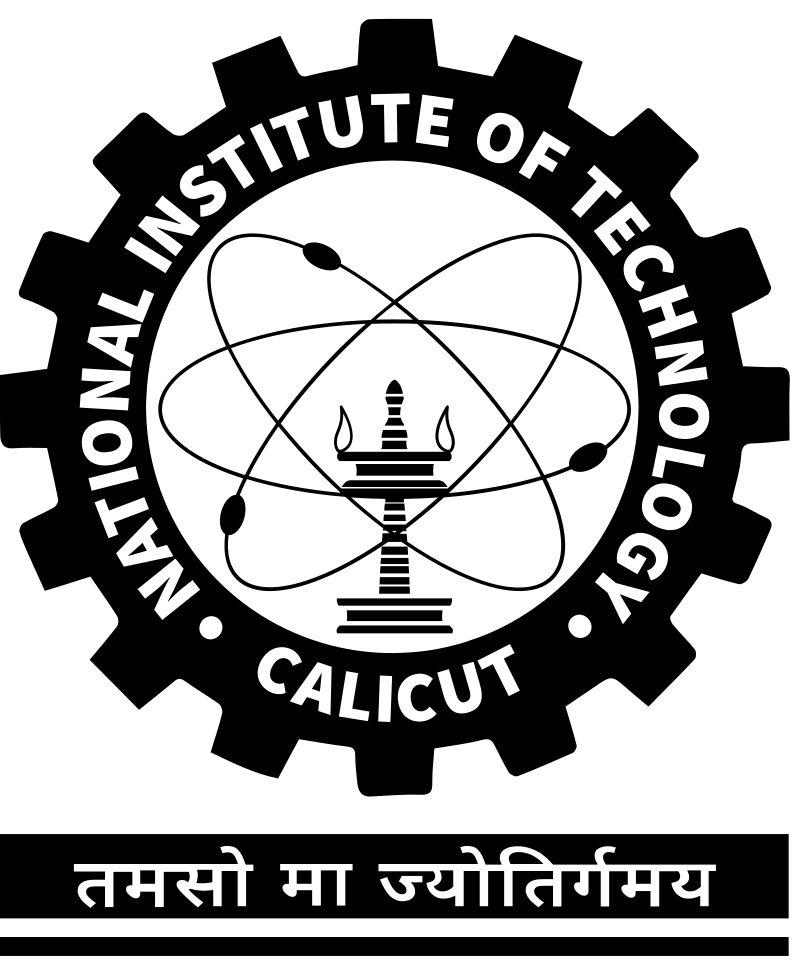
\includegraphics[scale=0.05]{imagens/nitc_logo.png}} 
\institute[]{Centre for Information Technology Research and Automation\par National Institute of Technology Calicut} 


\usepackage[utf8]{inputenc}
\usepackage[english]{babel}
\usepackage[T1]{fontenc}

\usepackage{amsmath}
\usepackage{amsfonts}
\usepackage{amssymb}
\usepackage{graphicx}



\begin{document}
	\begin{frame}
		\titlepage
	\end{frame}
	
	\begin{frame}
		\section{Outline}
		\frametitle{Outline}
		\begin{itemize}
			\item Day I
			\begin{itemize}
				\item Introduction to Libre and Linux
				\item Introduction to Ubuntu Desktop
			\end{itemize}
			\item Day II
				\begin{itemize}
					\item File Management
					\item Regular Expressions
				\end{itemize}		
			\item Day III
				\begin{itemize}
					\item Shell Scripting
					\item Linux in Daily Life
				\end{itemize}
		\end{itemize}
	\end{frame}
	
	\begin{frame}
		\section{Introduction to Libre and Linux}
		\frametitle{Introduction to Libre and Linux}
		\begin{itemize}
			\item A brief history of Unix
			\item GNU - GNU is Not Unix - Richard Stallman
			\item Linux - Linus Torvalds
			\item Why is it important? 
		\end{itemize}
		
	\end{frame}

\end{document}